\section{Motivation}
Um eine Motivation zu schreiben habe ich ChatGPT um Hilfe gebeten. 
Da es mir keine sinnvolle Antwort geben konnte,
muss ich jetzt tatsächlich selber zu Wort kommen.\\
Frodo und Sam stiegen den Vulkan empor um sie brannte die Erde. Sie waren so weit gekommen um den Ring zu zerstören, dass
sie dieser Berg nicht aufhalten würde. Sie hatten es geschafft.
Als sie in das Innere des Vulkan vorstießen stellte sich ihnen Gollum entgegen.
Ein verwarlostes Wesen welches Jahre lang in Besitz des Rings war. ``Mein Schatz'' rief er.
"Nein er muss zerstört werden" erwiederte Sam. Frodos körper war schwer, der Ring um seinen Hals machte Laufen schwer.
Ein erbitterter Kampf entfachte um Leben und Tod, unter ihnen brodelte die Lava. Schöließlich fiel Gollum die Falswand hinab und mit ihm der Ring.
Als dieser die LAva berührte passierte nichts.\\
\[Warum ?\]
Die beiden hatten vergessen die Temperatur der Lava zu bestimmen denn sie war zu kalt um den Ring zu schmelszen. Wie konnte ihnen das passieren? Dabei gibt
es viele gute Methoden dies zu tun, manche sind besser als andere. Um das herauszufinden
wird in dem folgenden Versuch das Messverhalten von Thermometern wie dem Pt-100, dem Gasthermometer, dem Thermoelement, dem Pyrometer und einem Flüssigkeitsthermometer untersucht.
Genaue Temperaturbestimmung ist in der Physik essentiell. Deshalb ist der Umgang mit Therometern ein zentrales Element dieses Versuchs.

\section{Messverfahren}

Zuerst wurde die Temperatur innerhalb einer Gasflame eine Bunsenbrenners, einmal bei leichtender und bei rauschender Flamme gemessen.
Und die Temperaturen der einzelnen Flammenteile aufgezeichnet.
Dabei durften wir den Bunsenbrenner trotz vorhandenen Führerscheins nicht anzünden.\\ \smallskip
Anschließend wurde ein Eiswasserbad aufgesetzt mit welchem das Gasthermometer und das Pt-100 Thermometer auf einen ersten
Fixpunkt geeicht wurden. Danach wurde die Temperatur schrittweise erhöht und die Messwerte aller Thermometer notiert.\\
Schließlich konnte bei dem Siedepunkt ein zweiter Fixpunkt erstellt werden\\ \smallskip
Zuletzt wurden die Thermometerwerte der Siedepunkte von Stickstoff und einer $CO_2$-Alkohol Lösung bestimmt.

\subsection{Gasthermometer}
Ein Gasthermometer besteht aus einem Glasballon, der mit Luft gefüllt ist und einem Barometer.
Diese sind über einen Glashalmverbunden. In dem Glasha.m bleibt die Tmperatur nahezu auf Raumteperatur,
was dafür sorgt, das die Luft in diesem nach Temperaturänderung des Glasballons komprimiert bzw. expandiert wird.
Das Barometer kann diese Druckänderung messen. Da Luft als nahezu Ideales Gas betrachtet werden kann gilt:

\begin{equation}
    p = NkT
\end{equation}

Weshlab gilt $p \propto T$. Daraus kann dann die Temperatur bestimmt werden.

\subsection{Thermoelement}
Das Thermoelement funktioniert über den Seebeck-Effekt. Dieser besagt,
dass an der Kontaktfläche zweier Metallen mit unterschiedlichen Austrittsarbeiten
eine Spannung, in Abhänigigkeit der Temperatur an der Kontaktfläche und der Twmperatur an den Enden der Metalle, induziert wird. 
Aus dieser Spannung kann dann eine relative Temperatur bestimmt werden.
Verwendet wird in dem Versuch ein Platin-Rhodium Thermoelement.

\subsection{Pt-100 Thermometer}
Das Pt-100 Thermometer funktioniert über einen Temperaturabhängigen Platinwiderstand.
Bei diesen wird ein kleiner Strom von 1 mA angelegt, damit möglichst wenig Eingenwärme erzeugt wird.
Aus dem Spannungsanstieg bzw Abfall kann dann die relative Temperatur bestimmt werden.
Der Zusammenhang zwischen Widerstand und Spannung wird durch das folgende Polynom beschrieben: 
\begin{equation}
    R(T) = R_{0} \left( 1 + A T + B T^{2} \right),
    \label{eq:Polynom}
\end{equation}
mit den Koeffizienten
\begin{align*}
    A &= 3{,}9083 \times 10^{-3}\,[^\circ\mathrm{C}^{-1}] \\
    B &= -5{,}775 \times 10^{-7}\,[^\circ\mathrm{C}^{-2}].
\end{align*}
Im Temperaturbereich $0-100 1^\circ C$ kann dieser Zusammenhang näherungsweise als linear betrachtet werden.

\subsection{Flüssigkeitsthermometer}
Das Flüssigkeitsthermometer ist das klassische Haushaltsthermometer. Dort wird die Temperatur durch die
Ausdehnung einer Flüssigkeit unter Temperaturänderung betrachtet. Die Temperatur kann dann an des Spiegels der ausgedehnten Flüssigkeit abgelesen werden.

\subsection{Pyrometer}
Körper, dessen einer Temperatur $>0K$ beträgt, sendet Wärestrahlung aus.
Ein Pyrometer misst die von einem Körper ausgehende Strahlungsleistung zur Temperaturbestimmung.

\begin{equation}
    P = \epsilon(T) \sigma A T^4
\end{equation}

Wobei A die strahlende Fläche, $\sigma$ die Stefan-Bolzmannkonstante und $T$ die absolute Temperatur.
$\epsilon(T) < 1$ stellt den Faktor dar, der eine realen Körper von einem schwarzen Strahler unterscheidet.
Die eingesetzten pyrometer können Strahlung im Bereich von $8 \mu m$ bis $14 \mu m$ integrieren.

\newpage
\section{Versuchsskizze}
\begin{figure}[h!]
    \centering
    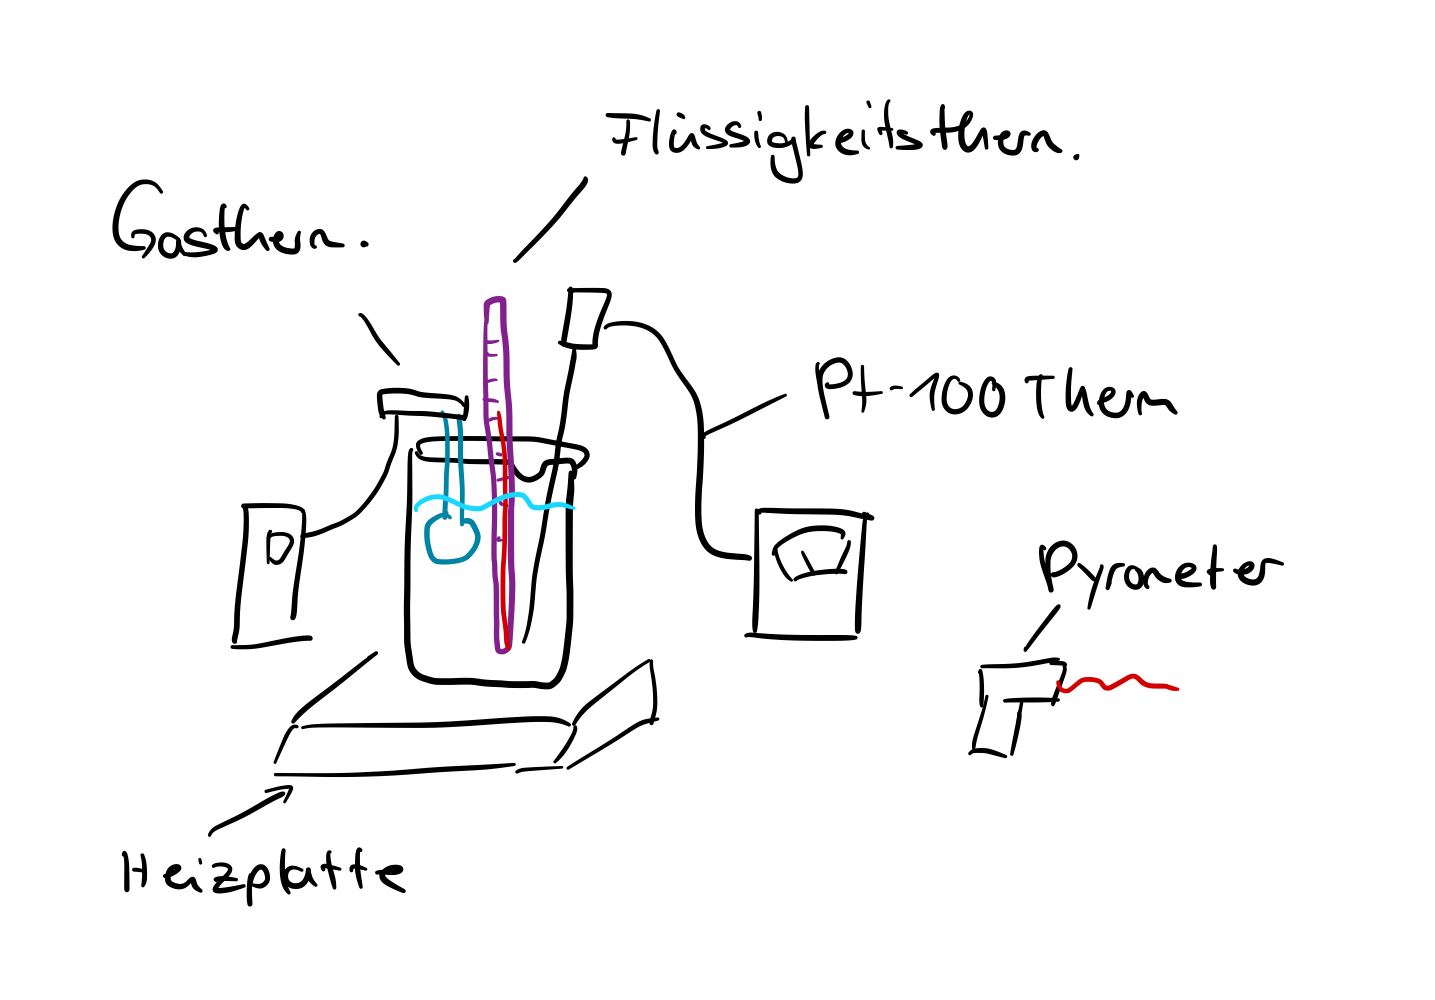
\includegraphics[width=.5\textwidth]{41Skizze.jpeg}
    \caption{Skizze Temperaturmessung Wasser}
\end{figure}
\begin{figure}[h!]
    \centering
    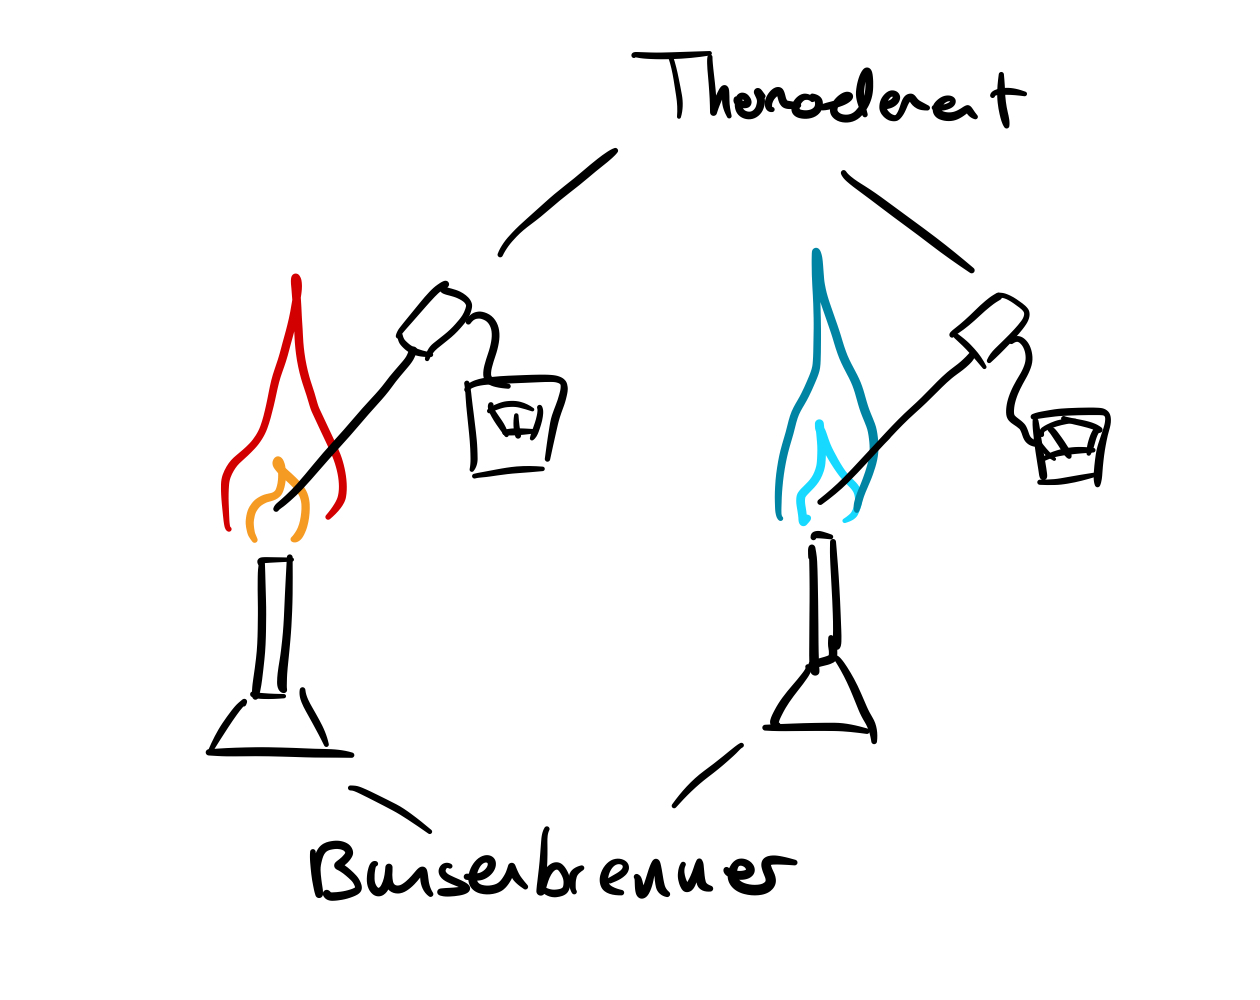
\includegraphics[width=.5\textwidth]{41Theroel.jpeg}
    \caption{Skizze Temperaturmessung Bunsenbrenner}
\end{figure}

\section{Standartabweichung}
Allgemein lässt sich die Abweichung eines Messwertes $x$ zu einem Literaturwert $x_{Lit}$ darstellen durch die Sigmaabweichung:

\begin{equation}
    \frac{|x-x_{Lit}|}{\Delta x} = k \sigma \ \ mit \ k \in \mathbb{R}
    \label{eq:sigma}
\end{equation}